\documentclass[t]{beamer} 
\usepackage{tikz}
\usepackage[all]{xy}
\usepackage{amsmath,amssymb}
\usepackage{hyperref}
\usepackage{graphicx}
\usepackage[noend]{algcompatible}
\usepackage{multirow}

\DeclareMathOperator*{\argmin}{arg\,min}
\DeclareMathOperator*{\Lik}{Lik}
\DeclareMathOperator*{\PoissonLoss}{PoissonLoss}
\DeclareMathOperator*{\Peaks}{Peaks}
\DeclareMathOperator*{\Segments}{Segments}
\DeclareMathOperator*{\argmax}{arg\,max}
\DeclareMathOperator*{\maximize}{maximize}
\DeclareMathOperator*{\minimize}{minimize}
\newcommand{\sign}{\operatorname{sign}}
\newcommand{\RR}{\mathbb R}
\newcommand{\ZZ}{\mathbb Z}
\newcommand{\NN}{\mathbb N}
\newcommand{\z}{$z = 2, 4, 3, 5, 1$} 

\newcommand{\algo}[1]{\textcolor{#1}{#1}}
\definecolor{PDPA}{HTML}{66C2A5}
\definecolor{CDPA}{HTML}{FC8D62}
\definecolor{GPDPA}{HTML}{4D4D4D}

% Set transparency of non-highlighted sections in the table of
% contents slide.
\setbeamertemplate{section in toc shaded}[default][100]
\AtBeginSection[]
{
  \setbeamercolor{section in toc}{fg=red} 
  \setbeamercolor{section in toc shaded}{fg=black} 
  \begin{frame}
    \tableofcontents[currentsection]
  \end{frame}
}

\begin{document}

\title{Classification of imbalanced labeled data with AUM loss}

\author{
  Toby Dylan Hocking --- toby.hocking@nau.edu\\
  Acronis SCS and Northern Arizona University, USA\\
  School of Informatics, Computing and Cyber Systems\\
  Machine Learning Research Lab --- \url{http://ml.nau.edu}\\
  \includegraphics[height=3.5cm]{2021-03-lab-ski-lunch} \\
  joint work with Joseph R. Barr, Garinn Morton, Tyler Thatcher, and Peter Shaw.\\
}

\date{}

\maketitle

\section{Problem Setting: imbalanced supervised  binary classification}

\begin{frame}
  \frametitle{Problem: unbalanced supervised binary classification}
  
  \begin{itemize}
  \item Given pairs of inputs $\mathbf x\in\mathbb R^p$ and outputs
    $y\in\{0,1\}$ can we learn a score 
    $f(\mathbf x)\in\mathbb R$, predict $y=1$ when $f(\mathbf x)>0$?
  \item Example: email, $\mathbf x =$bag of words, $y=$spam or not.
  \item Example: code, $\mathbf x =$embedding, $y=$vulnerable or not.
  \item Example: images. Jones {\it et al.} PNAS 2009.
  \item In all of these examples, we typically have many more negative
    examples than positive examples (unbalanced).
    \parbox{1.5in}{\includegraphics[width=1.5in]{cellprofiler}}
    \parbox{2.4in}{Most algorithms (Logistic regression, SVM, etc) minimize a differentiable surrogate of zero-one loss = sum of:\\
      \textbf{False positives:} $f(\mathbf x)>0$ but $y=0$ (predict
      budding, but cell is not).\\
      \textbf{False negatives:} $f(\mathbf x)<0$ but $y=1$ (predict
      not budding, but cell is).
  }
  \end{itemize} 
\end{frame}

\begin{frame}
  \frametitle{Receiver Operating Characteristic (ROC) Curves}
  \begin{itemize}
  \item Classic evaluation method from the signal processing
    literature (Egan and Egan, 1975).
  \item For a given set of predictions, plot True Positive Rate
    (=1-False Negative Rate) vs False Positive Rate, each point on the
    ROC curve is a different threshold of the predicted scores.
  \item Best classifier has a point near upper left (TPR=1, FPR=0), with large
    Area Under the Curve (AUC).
  % \item Proposed idea: a new surrogate for AUC that is differentiable,
  %   so can be used for gradient descent learning.
  \end{itemize}
  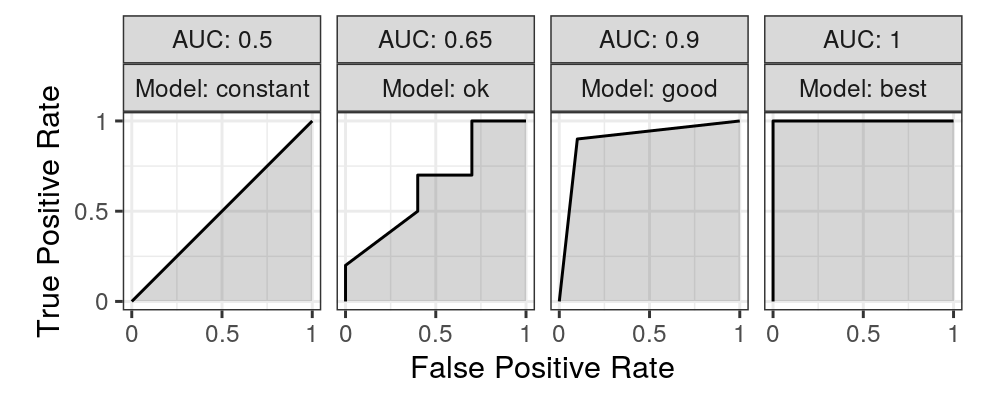
\includegraphics[width=\textwidth]{figure-more-than-one-binary}
\end{frame}

\begin{frame}
  \frametitle{Research question and new idea}
  Can we learn a binary classification function $f$ which directly
  optimizes the ROC curve?
  \begin{itemize}
  \item Most algorithms involve minimizing a differentiable surrogate
    of the zero-one loss, which is not the same.
  \item The Area Under the ROC Curve (AUC) is piecewise constant
    (gradient zero almost everywhere), so can not be used with
    gradient descent algorithms.
  \item We propose to encourage points to be in the upper left of ROC
    space, using a loss function which is a differentiable surrogate
    of the sum of min(FP,FN).
  \end{itemize}
  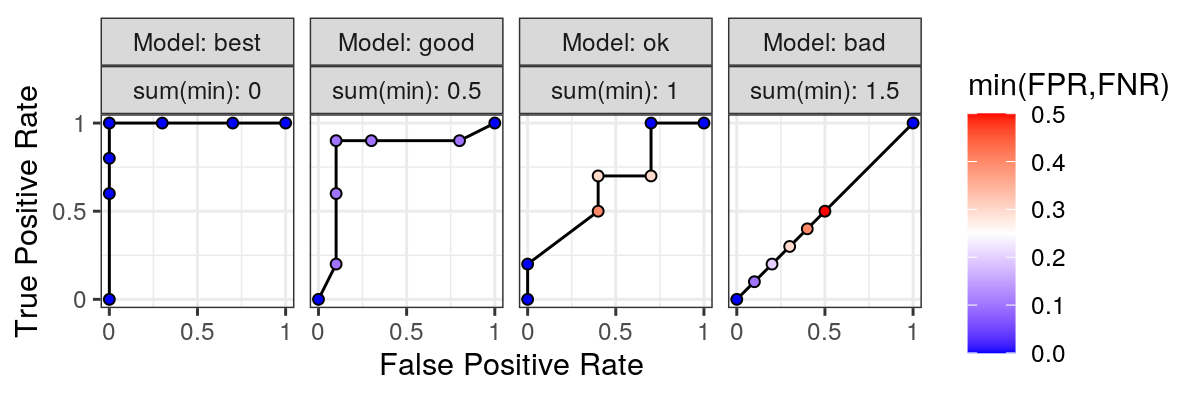
\includegraphics[width=\textwidth]{figure-more-than-one-binary-dots}
\end{frame}

\section{Proposed surrogate loss for ROC curve optimization: Area Under Min\{FP,FN\} (AUM)} 

\begin{frame}
  \frametitle{Proposed method, details 1}
  \begin{itemize}
  \item Hillman J and Hocking TD, Optimizing ROC Curves with a
    Sort-Based Surrogate Loss for Binary Classification and
    Changepoint Detection, arXiv:2107.01285.
  \item  $n$ training examples $\{(x_i, y_i): x_i \in \mathbb{R}^p, y_i\in \{-1,+1\} \}_{i=1}^n$,
  \item prediction vector $\mathbf{\hat y}=[\hat y_1 \cdots \hat y_n]^\intercal\in\mathbb R^n$,
\item we compute the following false positive and false negative totals for each example $i\in\{1,\dots,n\}$,
  \end{itemize}
\begin{equation}
  \text{FP}_i = \sum_{j: \hat y_j \geq \hat y_i} I[y_j = -1], \ \ 
  \text{FN}_i = \sum_{j: \hat y_j \leq \hat y_i} I[y_j = 1].\label{eq:fp-fn-under}
\end{equation}
$\text{FP}_i, \text{FN}_i$ are the error values at
the point on the ROC curve that corresponds to observation $i$.
\end{frame}

\begin{frame}
  \frametitle{Proposed method, details 2}
  \begin{itemize}
  \item Sort the observations by predicted value $\hat y_i$ (log-linear time).
  \item yields a permutation $\{s_1,\dots, s_n\}$ of the indices $\{1,\dots,n\}$,
  \item so for every $q\in\{2,\dots,n\}$ we have
    $\hat y_{s_{q-1}} \geq \hat y_{s_q}$.
  \item Error values $\text{FP}_i,\text{FN}_i$ from last slide
    computed via modified cumulative sum (linear time).
  \item $q$ is index of points on the ROC curve, proposed loss is Area
    Under Min of FP and FN,
  \end{itemize}
\begin{equation}
    \text{AUM}(\mathbf{\hat y}) =
    \sum_{q=2}^n 
    (\hat y_{s_{q-1}} -\hat y_{s_q}) 
    \min\{
    \text{FP}_{s_q}, 
    \text{FN}_{s_q}\label{eq:min_below}
    \}. 
  \end{equation}

  Algorithm for computing proposed loss is log-linear, $O(n\log n)$.


\end{frame}
 

\begin{frame}
  \frametitle{Small AUM is correlated with large AUC} 
  
  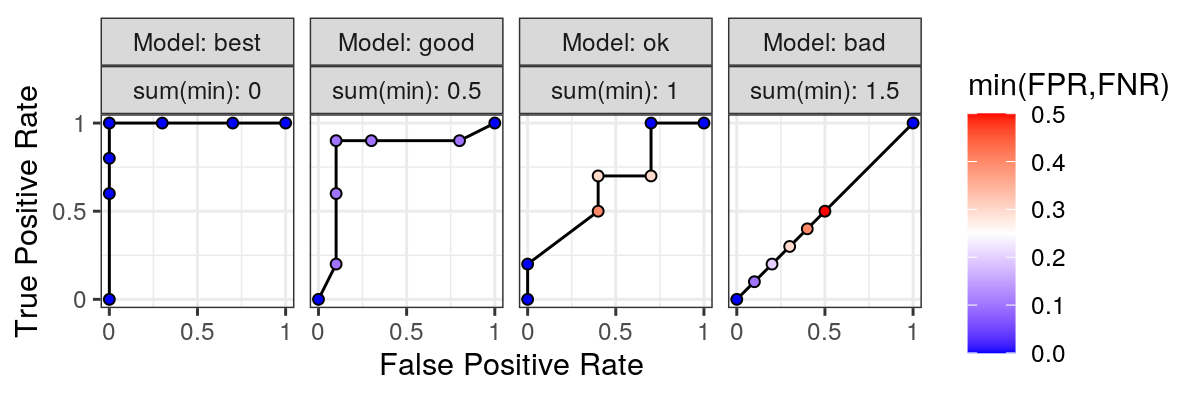
\includegraphics[height=1.5in]{figure-more-than-one-binary-dots}

  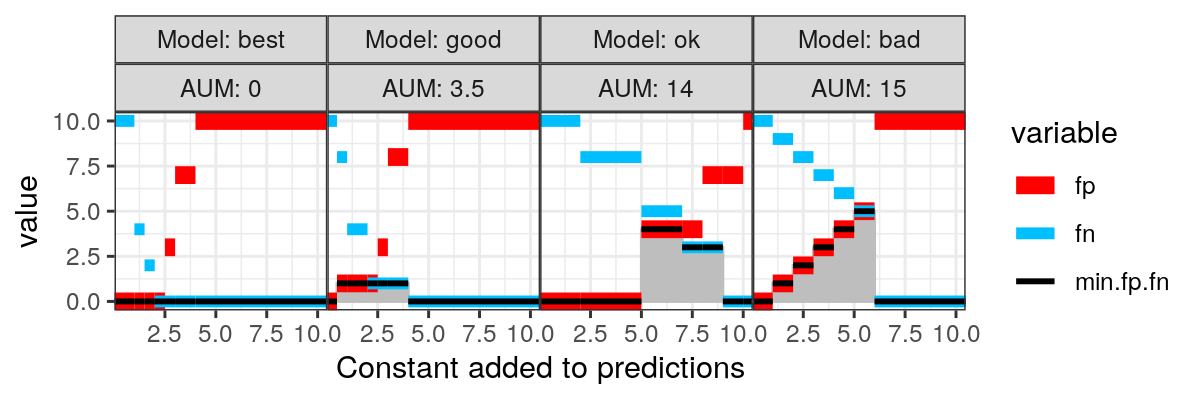
\includegraphics[height=1.5in]{figure-more-than-one-binary-aum}

  Grey area is proposed loss, Area Under Min (AUM).
  
\end{frame}

\begin{frame}
  \frametitle{Geometric interpretation of proposed loss}
  
    \centering
    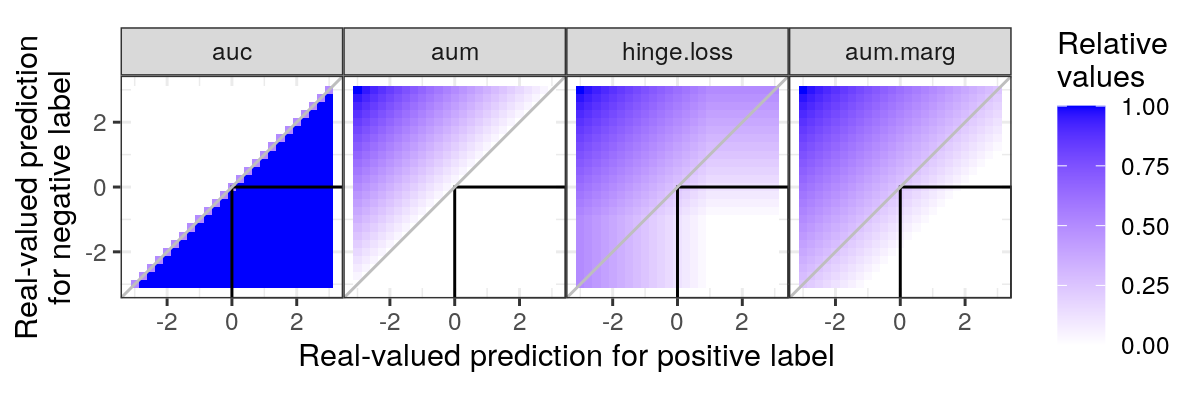
\includegraphics[width=0.8\textwidth]{figure-compare-hinge-loss}

    \begin{itemize}
    \item Visualization of loss functions when there are two labels: one
      positive, one negative.
    \item AUC is piecewise constant (abrupt changes 0--0.5--1),\\
      gradient is zero, can not be used for learning.
    \item AUM is differentiable almost everywhere,\\
      gradient can be used for learning.
    \item Min AUM happens when max AUC, correct rank (prediction
      for positive label greater than for negative).
    \item Min logistic loss encourages correct labels. 
    \end{itemize}
\end{frame}

\section{Empirical results: minimizing AUM results in maximizing AUC} 

% \begin{frame}
%   \frametitle{Data set sizes}
% \centering
% \begin{tabular}{l | r | r | r  | r | r | r}
% \hline
% & \texttt{ Android  } & \texttt{Android } & \texttt{ Linux } & \texttt{ OpenSSL } \ \  & \textsc{ Total } \\
% \textsc{ Language } \ \ & C & Java & C & C & \text{  C/Java  }
% \\
% \hline
% Non-CVE & 1,099,278 &	 1,143,050 & 562,841 & 	14,124	 & 2,819,293 \\
% CVE & 15,602 & 	1,288  & 22,260 & 107 &	39,257 \\
% \textbf{Total} & 1,114,880	& 1,144,338	& 585,101	& 14,231 & 2,858,550 \\
% \hline 
% \end{tabular}
% \end{frame}

% \begin{frame}
%   \frametitle{AUM gradient descent results in increased train AUC for
%     a real changepoint problem}

% 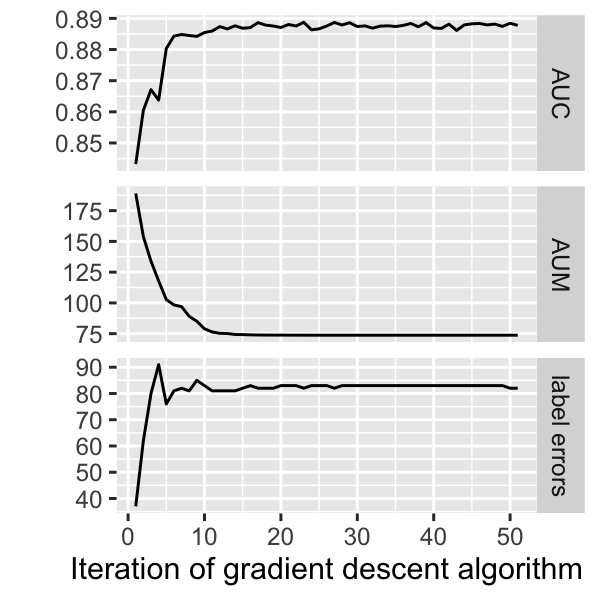
\includegraphics[height=3.7cm]{figure-aum-optimized-iterations.png}
% \includegraphics[height=3.7cm]{figure-aum-train-both.png}

% \begin{itemize}
% \item Left/middle: changepoint problem initialized to prediction vector with
%   min label errors, gradient descent on prediction vector.
% \item Right: linear model initialized by minimizing regularized convex
%   loss (surrogate for label error, Hocking \emph{et al.} ICML 2013),
%   gradient descent on weight vector.
% \end{itemize}

% \end{frame}

% \begin{frame}
%   \frametitle{Learning algorithm results in better test AUC/AUM for changepoint problems}
    
% \includegraphics[width=\textwidth]{figure-test-aum-comparison.png}
% \includegraphics[width=\textwidth]{figure-test-auc-comparison.png}

% \begin{itemize}
% \item Five changepoint problems (panels from left to right).
% \item Two evaluation metrics (AUM=top, AUC=bottom).
% \item Three algorithms (Y axis), Initial=Min regularized convex loss
%   (surrogate for label error, Hocking \emph{et al.} ICML 2013), Min.Valid.AUM/Max.Valid.AUC=AUM
%   gradient descent with early stopping regularization.
% \item Four points = Four random initializations.
% \end{itemize}

% \end{frame}

\begin{frame}
  \frametitle{Standard logistic loss fails for highly imbalanced labels}

 \includegraphics[width=\textwidth]{figure-unbalanced-grad-desc-logistic.png}

 \begin{itemize}
 \item Subset of zip.train/zip.test data (only 0/1 labels).
 \item Test set size 528 with balanced labels (50\%/50\%).
 \item Train set size 1000 with variable class imbalance.
 \item Loss is $\ell[f(x_i), y_i]w_i$ with $w_i=1$ for identity
   weights, $w_i=1/N_{y_i}$ for balanced, ex: 1\% positive means
   $w_i\in\{1/10,1/990\}$.
 \end{itemize}

\end{frame}

\begin{frame}
  \frametitle{Linear learning algorithms in unbalanced image data}

 \includegraphics[width=\textwidth]{figure-unbalanced-grad-desc.png}

 \begin{itemize}
 \item Zip data set (digits), 16x16 images, ten classes, only use 0/1.
 \item Imbalanced train set with 1000 images (discard some data).
 \item Balanced test: 528 images overall (264 of each class).
 \item Linear model, full gradient, early stopping regularization.
 \item Squared hinge all pairs is a classic/popular surrogate loss function
   for AUC optimization. (Yan \emph{et al.} ICML 2003)
 \end{itemize}

\end{frame}

\begin{frame}
  \frametitle{Neural network with stochastic gradient and a time budget}

 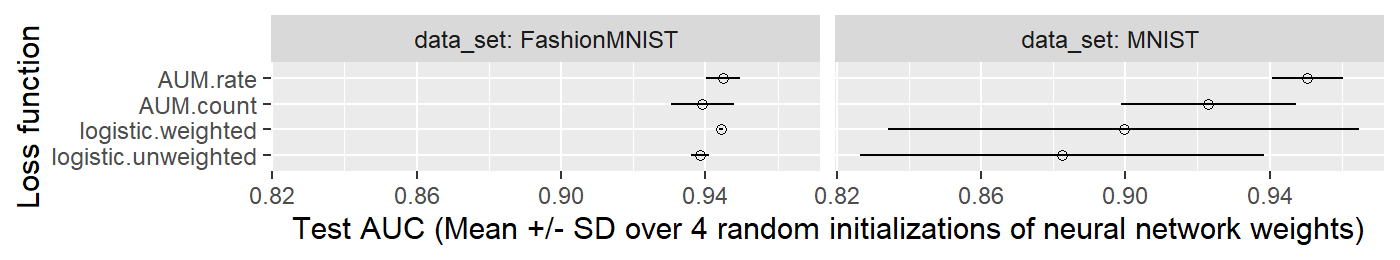
\includegraphics[width=\textwidth]{figure-aum-neural-networks-test-auc.png}

 \begin{itemize}
 \item (Fashion)MNIST data, 28x28 images, binarized ten class problem
   (0-4:negative, 5-9:positive).
 \item Unbalanced train set with 300 positive, 30,000 negative
   examples ($\approx$1\% positive).
 \item Balanced test set of 10,000 images ($\approx$50\% positive).
 \item LeNet5 convolutional network, average pooling, ReLU
   activation, batch size 1000, max 10 epochs, early stopping.
 \item AUM.rate: area under min(FPR,FNR), rates in [0,1].
 \item AUM.count: area under min(FP,FN), number of errors.
 \item Proposed AUM losses similar to/better than logistic loss.
 \end{itemize}

\end{frame}

\begin{frame}
  \frametitle{Proposed AUM has nearly linear computation time}

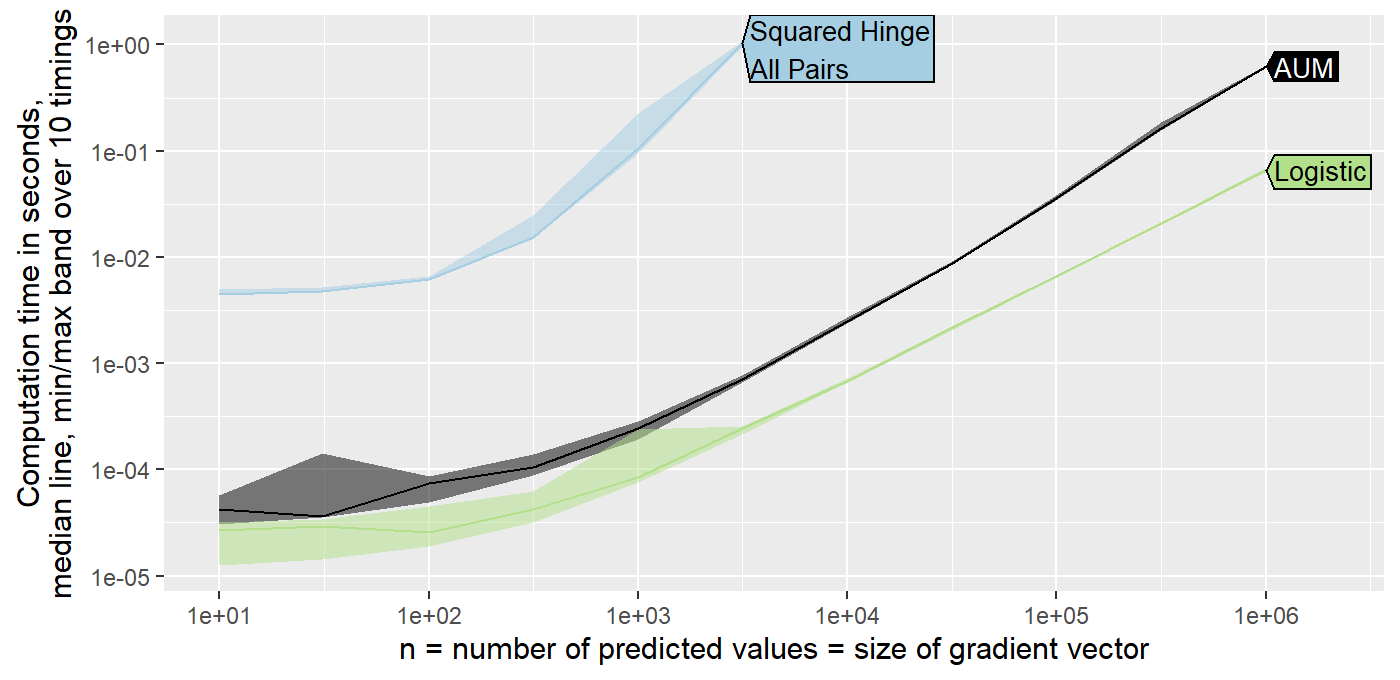
\includegraphics[width=\textwidth]{figure-aum-grad-speed-binary.png}

\begin{itemize}
  \item Log-log plot, so slope indicates time complexity class.
\item Logistic $O(n)$. 
\item AUM $O(n\log n)$. (proposed)
\item Squared Hinge All Pairs $O(n^2)$. (Yan \emph{et al.} ICML 2003)
\end{itemize}
  
\end{frame}
\section{Discussion and Conclusions}

\begin{frame}
  \frametitle{Discussion and Conclusions}
  \begin{itemize}
  \item ROC curves are used to evaluate binary classification
    algorithms, especially with unbalanced labels.  
  \item We propose a new loss function, AUM=Area Under Min(FP,FN),
    which is a differentiable surrogate of the sum of Min(FP,FN) over
    all points on the ROC curve.
  \item We propose new algorithm for efficient log-linear AUM and directional
    derivative computation.
  \item Implementations available in R/C++ and python/torch:
    \url{https://cloud.r-project.org/web/packages/aum/}
    \url{https://tdhock.github.io/blog/2022/aum-learning/}
  \item Empirical results provide evidence that learning using AUM
    minimization results in maximizing Area Under ROC Curve.
  \item Future work: exploiting piecewise linear structure of the AUM
    loss, other model classes, other problems/objectives.
  \end{itemize}
\end{frame}

\begin{frame}
  \frametitle{Thanks and come visit the ML lab in Flagstaff!}

  \includegraphics[height=3in]{2021-03-lab-ski-lunch} 

  Contact: toby.hocking@nau.edu

\end{frame} 

\end{document}
